\section{概论}

\begin{frame}[fragile]
  \frametitle{概论}

  \begin{easylist}
    & 计算机程序设计和数据处理的理论与技术基础
    & 核心内容:
    && 线性表、栈和队列、字符串、树与森林、图、排序、查找
    & 目标
    && 掌握数据结构的特点、存储方法和基本运算
    && 初步掌握算法的时间和空间分析技术
    && 能够针对不同数据对象的特性,选择适当的数据结构和存储结构以及相应的算法
  \end{easylist}
\end{frame}

\begin{frame}[fragile]
  \frametitle{课程信息}
  \begin{easylist}
    & 教室安排:信息楼403; 上课时间:周四16:00 -- 17:30
    & 教学方式
    && 课堂教学与演示(听讲、看书、练习)
    && 上机练习
    & 平时成绩:
    && 课程作业:50\%
    && 研讨交流与发言情况:30\%
    && 课堂提问:10\%
    && 考勤:10\%
    & 最终成绩:
    && 随堂闭卷考试(50\%) + 平时成绩(50\%)
    &  要求独立完成作业,切勿抄袭!
  \end{easylist}
\end{frame}

\begin{frame}[fragile]
  \frametitle{学习建议}
  \begin{easylist}
    & 教材
    && 严蔚敏,吴伟民. 《数据结构(C语言版)》,清华大学出版社. (国内经典教材,写作严谨,广泛使用。)
    && 算法导论
    && 大话数据结构
    & 在线课程
    & 编程语言
    && 选择一种作为实践语言:Java、Python(根据同学们反馈选择)
    && 能够看懂不同编程语言的代码
    && 伪代码(Pseudocode)
    &&& 一种非正式,类似于英语结构,用于描述模块结构图的语言。
  \end{easylist}
\end{frame}

\begin{frame}[fragile]
  \frametitle{1997年的人机大战}

  \begin{columns}
    \begin{column}[T]{.5\linewidth}
      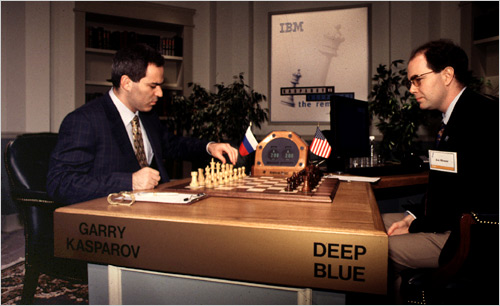
\includegraphics[width=0.8\textwidth]{figs/intro/deep_blue_1.png}

        1997年5月11日,国际象棋世界冠军卡斯帕罗夫与IBM公司的超级电脑深蓝(Deep Blue)对弈。
    \end{column}
    \begin{column}[T]{.5\linewidth}
      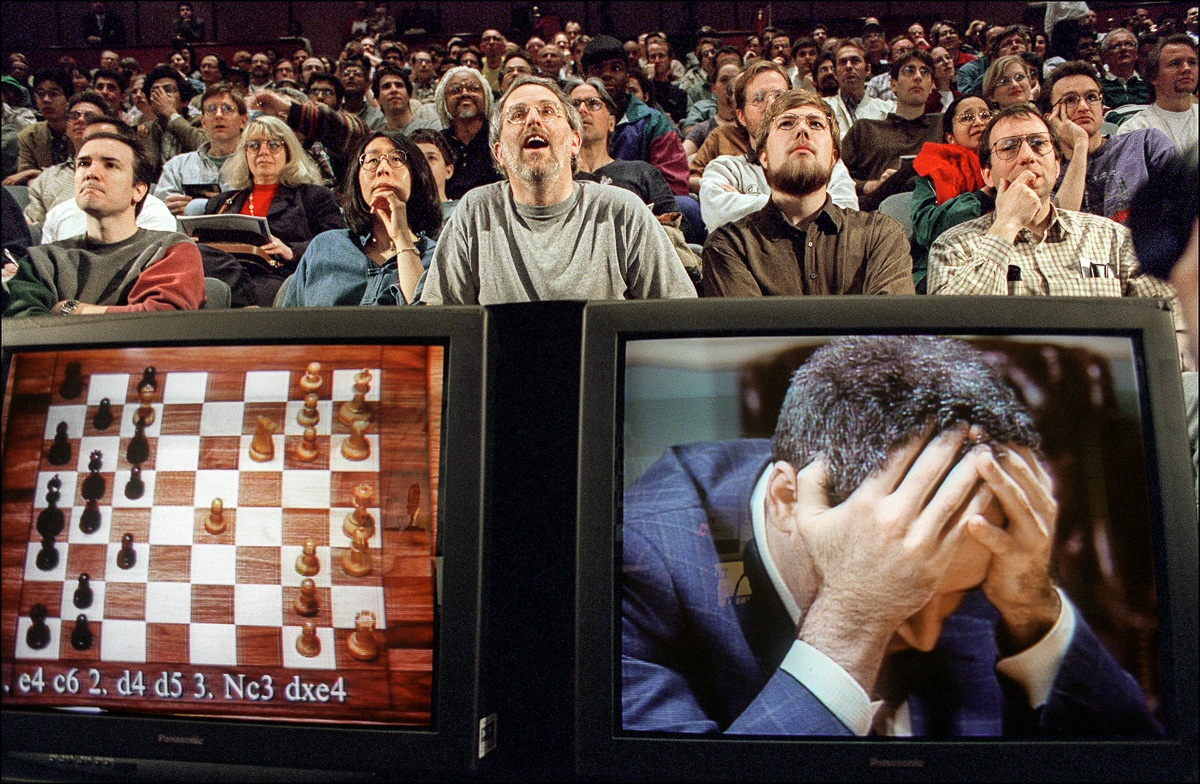
\includegraphics[width=0.8\textwidth]{figs/intro/deep_blue_2.png}

      棋迷在纽约通过电视观战。当日,卡斯帕罗夫在纽约再次负于深蓝,从而在当年的
      “人机大战”中以一胜二负三和的战绩败北。
    \end{column}
  \end{columns}
\end{frame}

\begin{frame}[fragile]
  \frametitle{~}
  \begin{columns}
    \begin{column}[T]{.65\linewidth}
      \begin{enumerate}
      \item “深蓝”重量达1.4吨,有32个CPU,每个CPU有8块专门为进行国际象棋对弈设计
        的处理器,平均运算速度为每秒200万步。总计256块处理器集成在IBM研制的
        RS6000/SP并行计算系统中,从而拥有每秒超过2亿步的惊人速度。

      \item IBM研制小组向“深蓝”输入了100年来所有国际特级大师开局和残局的下法。美
        国特级大师本杰明将他对象棋的理解编成程序教给“深蓝”。虽不会思考,但它无穷
        无尽的计算能力在很大程度上弥补了这一缺陷。
      \end{enumerate}
    \end{column}
    \begin{column}[T]{.3\linewidth}
      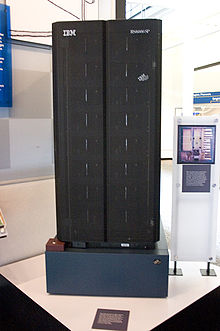
\includegraphics[width=0.8\textwidth]{figs/intro/deep_blue_3.png}
    \end{column}
  \end{columns}
\end{frame}

\begin{frame}[fragile]
  \frametitle{~}
  \begin{columns}
    \begin{column}[T]{.65\linewidth}
      \begin{enumerate}
      \item 模型: 棋盘、棋子的表示
      \item 算法: 对弈的规则和策略
        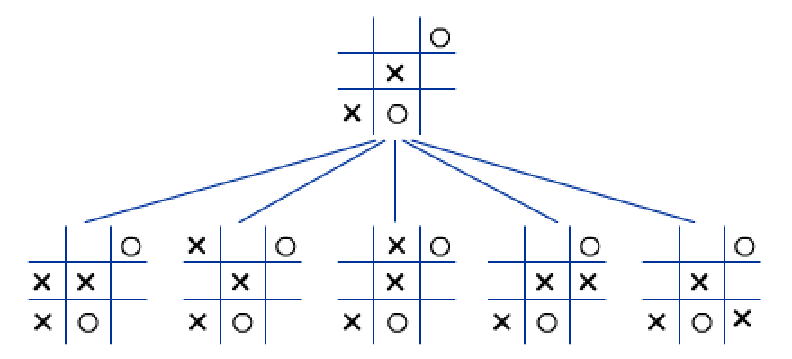
\includegraphics[width=0.8\textwidth]{figs/intro/chess_2.png}
      \item 对弈的本质即在该空间里进行有效的搜索
      \end{enumerate}
    \end{column}
    \begin{column}[T]{.3\linewidth}
      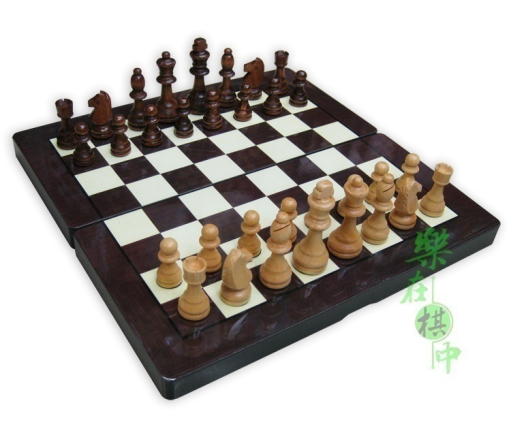
\includegraphics[width=0.8\textwidth]{figs/intro/chess_1.png}
    \end{column}
  \end{columns}
\end{frame}

\begin{frame}[fragile]
  \frametitle{~}

  \begin{columns}
    \begin{column}[T]{.5\linewidth}
      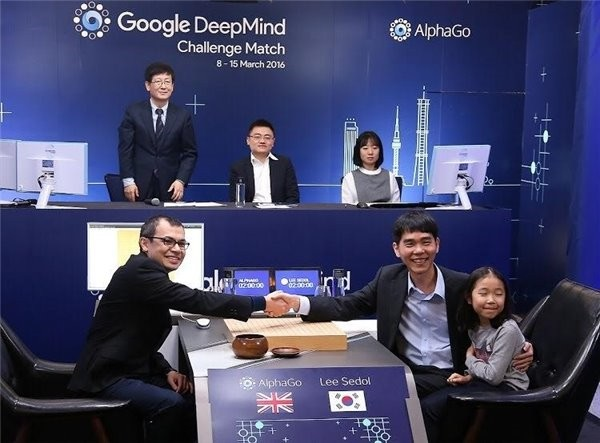
\includegraphics[width=0.8\textwidth]{figs/intro/alphago_1.png}

      2016年3月9日,Google旗下的AlphaGo电脑击败韩国九段棋手李世石。
    \end{column}
    \begin{column}[T]{.5\linewidth}
      
\includegraphics[width=0.8\textwidth]{figs/intro/alphago_2.png}

      2017年5月27日,世界排名第一的人类棋手柯洁负于AlphaGo,人机大战2.0定格在了0:3。
    \end{column}
  \end{columns}
\end{frame}

\begin{frame}[fragile]
  \frametitle{~}

  \begin{itemize}
  \item 对于擅长于计算的计算机来说,围棋的难度在很大程度上来自于19*19路棋盘背后
    所蕴含的巨大的无法穷尽的变化( 3361种下法),这是基于“穷尽法”的“深蓝”无法在
    围棋上战胜人类的原因。

  \item AlphaGo取得如此成绩,关键是深度学习和类神经网络技术。
  \item AlphaGo将棋盘看作是一个19*19像素构成的图片,利用类似于卷积神经网络的技术
    预测下一步走法。
  \end{itemize}
\end{frame}

\begin{frame}[fragile]
  \frametitle{依赖于高效的搜索}

  \begin{itemize}
  \item 如何快速的搜索到右方的图例?
  \end{itemize}

    \begin{columns}
    \begin{column}[T]{.6\linewidth}
      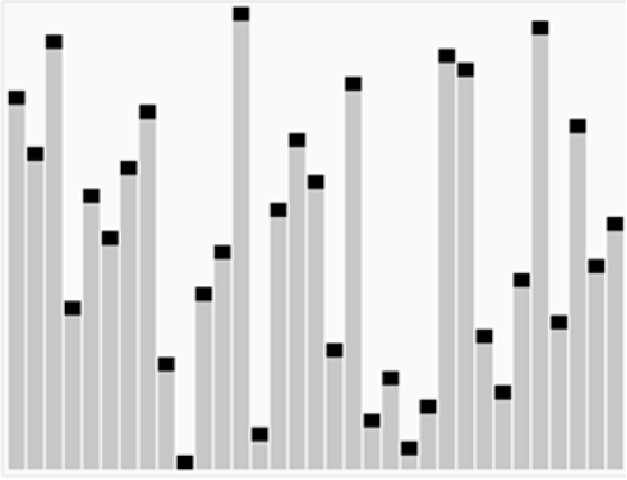
\includegraphics[width=0.8\textwidth]{figs/intro/sort_demo_1.png}
    \end{column}
    \begin{column}[T]{.5\linewidth}
      \vspace{2cm}
      
\includegraphics[width=0.2cm]{figs/intro/sort_demo_2.png}
    \end{column}
  \end{columns}

\end{frame}

\begin{frame}[fragile]
  \frametitle{依赖于高效的搜索}

  \begin{itemize}
  \item 如何快速的搜索到右方的图例?
  \end{itemize}

    \begin{columns}
    \begin{column}[T]{.6\linewidth}
      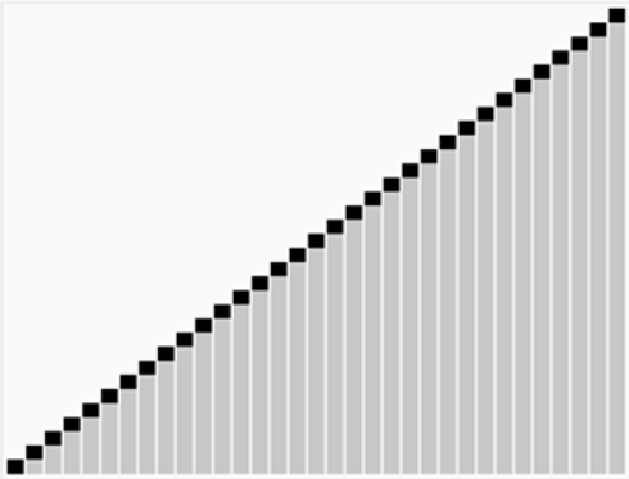
\includegraphics[width=0.8\textwidth]{figs/intro/sort_demo_3.png}
    \end{column}
    \begin{column}[T]{.5\linewidth}
      \vspace{2cm}
      
\includegraphics[width=0.2cm]{figs/intro/sort_demo_2.png}
    \end{column}
  \end{columns}

    数据有序有利于查找。需要对数据进行高效的组织/排序。
\end{frame}

\begin{frame}[fragile]
  \frametitle{Algorithms + Data Structures = Programs}

  \begin{easylist}
    & 算法
    && 处理问题的策略/操作步骤
    & 数据结构
    && 静态数据表示的数学模型(以及必须的操作)
    & 程序
    && 为计算机处理问题编制的一组指令集
  \end{easylist}

  \huge
  数据结构研究描述现实世界实体的数学模型及其上的操作在计算机中的表示和实现。
\end{frame}

\begin{frame}[fragile]
  \frametitle{FAQ}
  \begin{enumerate}
  \item 数据结构是又一门编程课吗?
  \item 不会C语言怎么办?
  \item 用别的语言学习数据结构可以吗?
  \item 怎样学好数据结构?
  \end{enumerate}
\end{frame}
